
\section{Introduction}

% TODO: mention history of foliations generally with pictures, then in birational geometry, classification, applications

Main reference: \cite{brunella_book}.

\section{Foliations and blowups}

% TODO: in this section we blah
% base field C
% Global geometry of foliation, line bundles K_F e.t.c. inform the geometry of the surface X
% Local geometry of foliation at singularities, models in A^2

\subsection{Foliations}

Suppose $X$ is a normal surface. To give a foliation $\scrF$ of $X$, we want to
define the tangent direction of the leaves of the foliation at any point in $X$,
giving a tangent vector up to scale at every point. We can accomplish this by
taking vector fields $v_i\in H^0(U_i,T_X)$ for an open cover $X=\cup_iU_i$, such
that $v_j=f_{ij}v_i$ for some non-vanishing holomorphic function
$f_{ij}\in H^0(U_i\cap U_j,\O_X^\times)$. Identifying data which would give rise
to the same foliation, we see that $\scrF$ is uniquely determined by the class
$\{f_{ij}\}$ in \v{C}ech cohomology $H^1(X,\O_X^\times)$, defining a line bundle
$T_\scrF$, and the global section $\{v_i\}$ of $T_\scrF^*\otimes T_X$ up to
multiplication by a nowhere vanishing holomorphic function.

\begin{example}
    Consider foliating $\A^2$ with horizontal leaves. The tangent direction for
    the leaves is generated by $\pdv{}{x}$, so $T_\scrF$ is trivial (as it must
    be on $\A^2$) with the section of $T_\scrF^*\otimes T_{\A^2}=T_{\A^2}$ given
    by $\pdv{}{x}$. Replacing $\pdv{}{x}$ by $-\pdv{}{x}$ or $2\pdv{}{x}$
    defines the same foliation.
    \begin{figure}[H]
        \centering
        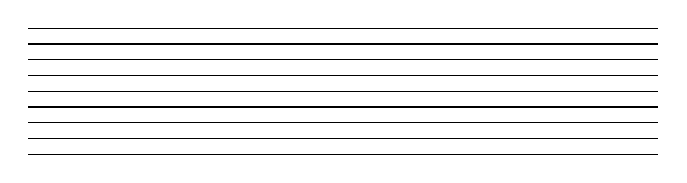
\begin{tikzpicture}
            \foreach \y in {-4,...,4}
                \draw (-4,\y*0.2) -- (4,\y*0.2);
        \end{tikzpicture}
        \caption{Fibration of $\A^2$ generated by $\pdv{}{x}$.}
    \end{figure}
\end{example}

We can also characterize the tangent spaces to the leaves as kernels of 1-forms,
leading to a similar definition with $T_X$ replaced by $\Omega^1_X$. The
foliation is given by a line bundle $N_\scrF^*$ and a global section
$\{\omega_i\}$ of $N_\scrF\otimes\Omega^1_X$ up to multiplication by a nowhere
vanishing holomorphic function.

\begin{example}
    The tangent vector $\pdv{}{x}$ on $\A^2$ is annhilated by the 1-form $dy$,
    and so the foliation from the previous example can also be seen as given by
    the trivial bundle $N_\scrF$ and the section $dy$ of
    $N_\scrF\otimes\Omega^1_{\A^2}$. We could construct $dy$ here by contracting
    $\pdv{}{x}$ with the area form $dx\wedge dy$, and so more generally the
    foliation generated by the vector field $A\pdv{}{x}+B\pdv{}{y}$ could also
    be specified by the contracted 1-form $Bdy-Adx$.
\end{example}

For a smooth foliation the tangent bundle $T_\scrF$ should be locally free, so
we would require that the vector fields $\{v_i\}$ (or the 1-forms
$\{\omega_i\}$) be non-vanishing. This is quite restrictive, and so in practice
we will be interested in foliations with singularities. We can also view the
above definitions as giving rational sections of $T_X$ or $\Omega^1_X$, defining
a global section after twisting by $\O(D)$ for $D$ a suitable divisor of poles.
There is a unique choice of $D$ such that the resulting section vanishes only in
codimension 2, and so we restrict our attention to foliations with singularities
in codimension 2.

\begin{example}
    Consider the extension of the foliation generated by $\pdv{}{x}$ on $\A^2$
    to $\P^2$. In coordinates $[1:y:z]$ the 1-form $dy$ on $\A^2$ becomes
    $d(y/z)=dy/z-ydz/z^2$, with a pole of order 2 along the hyperplane at
    infinity. Hence we get a section $(zdy-ydz)/z^2$ of $\Omega^1_{\P^1}(2)$
    which vanishes at $[1:0:0]\in\P^2$, defining a foliation $\scrF$ with
    $N_\scrF=\O(2)$ and a singularity at $[1:0:0]$. Note that the local form of
    the singularity is generated by the radial vector field
    $y\pdv{}{y}+z\pdv{}{z}$ annhilated by $zdy-ydz$, illustrated in
    \cref{fig:parallel}.
    \begin{figure}[H]
        \centering
        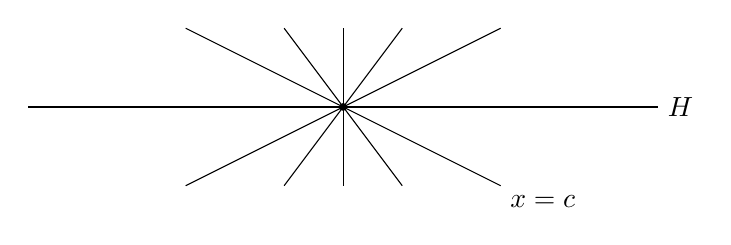
\begin{tikzpicture}
            \draw (-4,0)
                -- (0,0) node[circle,fill,inner sep=1pt] {}
                -- (4,0) node[anchor=west] {$H$};
            \draw (0,1) -- (0,-1);
            \draw (-0.75,-1) -- (0.75,1);
            \draw (0.75,-1) -- (-0.75,1);
            \draw (-2,-1) -- (2,1);
            \draw (2,-1) node[anchor=north west] {$x=c$} -- (-2,1);
        \end{tikzpicture}
        \caption{Parallel leaves converging at the horizon.}
        \label{fig:parallel}
    \end{figure}
\end{example}

The perspective of a foliation as the subsheaf $T_\scrF$ in $T_X$ leads us to a
general definition of foliations for higher dimensions.

\begin{definition}\label{defn:foliation}
    A rank $r$ foliation $\scrF$ of a normal variety $X$ is a rank $r$ subsheaf
    $T_\scrF$ of $T_X$ such that
    \begin{enumerate}[label=\roman*.]
        \item $T_X/T_\scrF$ is torsion-free,
        \item $T_\scrF$ is closed under the Lie bracket on $T_X$.
    \end{enumerate}
    The singular locus $\Sing(\scrF)$ is the singular locus of $X$ together with
    the locus where the stalks of $T_\scrF$ are not locally free submodules of
    the stalks of $T_X$.
\end{definition}

\begin{remark}
    Note that ii. is automatically satisfied for rank 1 foliations, as the Lie
    bracket then vanishes on $T_\scrF$. This condition is the requirement for
    integrability, leading to \cref{thm:frobenius}.
\end{remark}

See \cite[\S2]{friedman_book} for properties of torsion-free sheaves and
singularities of coherent sheaves. It follows that $T_X/T_\scrF$ is a subsheaf
of a locally free sheaf of the same rank, so in the case of a rank 1 foliation
on a surface we get $T_X/T_\scrF=I\cdot N_\scrF$ where $N_\scrF$ is a line
bundle and $I$ is the ideal sheaf cutting out $\Sing(\scrF)$. We then have two
dual exact sequences
\begin{equation}\label{eqn:tangent sequence}
    0 \to T_\scrF \to T_X \to I\cdot N_\scrF \to 0
\end{equation}
and
\begin{equation}\label{eqn:1-form sequence}
    0 \to N_\scrF^* \to \Omega^1_X \to I\cdot T_\scrF^* \to 0.
\end{equation}
Of course, the 1-forms vanishing on $T_\scrF$ are dual to $T_X/T_\scrF$,
justifying the re-use of the name $N_\scrF$ from above. The inclusion
$N_\scrF^*\to\Omega^1_X$ is given by the section of $N_\scrF\otimes\Omega^1_X$
defining the foliation.

We now restrict our attention to the case of a rank 1 foliation $\scrF$ on a
surface $X$.

\begin{proposition}\label{prop:canonical}
    $K_X=T_\scrF^*\otimes N_\scrF^*$.
\end{proposition}

\begin{proof}
    Non-vanishing sections of $K_X$ give by contraction an isomorphism between
    vector fields and 1-forms, identifying $T_\scrF$ and $N_\scrF^*$. In this
    way we get an isomorphism
    $K_X=\shHom(T_\scrF,N_\scrF^*)=T_\scrF^*\otimes N_\scrF^*$. This can also be
    seen from the exact sequence \cref{eqn:1-form sequence}, which restricts to
    an exact sequence of vector bundles on $U=X\setminus\Sing(\scrF)$, giving
    $K_X|_U=(N_\scrF^*\otimes T_\scrF^*)|_U$ by taking determinants, which
    implies the result because $\Sing(\scrF)$ has codimension at least 2.
\end{proof}

\begin{example}
    In the example of $\pdv{}{x}$ extended to $\P^2$ we had $N_\scrF=\O(2)$.
    Since $K_{\P^2}=\O(-3)$, the proposition gives $T_\scrF=\O(1)$, so
    $\pdv{}{x}$ should extend to a section of $T_{\P^2}(-1)$. Indeed in
    coordinates $[1:y:z]$ the pushforward of $\pdv{}{x}$ is
    $-z(y\pdv{}{y}+z\pdv{}{z})$, vanishing to first order at infinity.
\end{example}

\begin{definition}
    The \emph{canonical bundle} of the foliation $\scrF$ is
    $K_\scrF\coloneqq K_X\otimes N_\scrF=T_\scrF^*$.
\end{definition}

\begin{example}
    In the previous example $T_\scrF=\O(-1)$, so $K_\scrF=\O(1)$.
\end{example}

\subsection{Invariant curves}

To relate a foliation defined by a vector field or 1-form to the intuitive
notion of leaves foliating a surface, we have to consider its integral curves,
which give the leaves of the foliation. In general, the solutions to the
relevant differential equation will be analytic but not algebraic.

\begin{definition}
    If $(X,\scrF)$ is a foliated surface, a holomorphic curve $C$ in $X$ is
    \emph{invariant} under $\scrF$ if the inclusion $T_C\to T_X$ factors through
    $T_\scrF$.
\end{definition}

\begin{example}\label{ex:irrational saddle}
    Consider the foliation of $\A^2$ generated by $xdy+\sqrt2ydx$, corresponding
    to $x\pdv{}{x}-\sqrt2y\pdv{}{y}$. The differential equations defining an
    invariant curve are
    \begin{equation*}
        \dot x(t) = x(t), \quad \dot y(y)=-\sqrt2y(t).
    \end{equation*}
    There are two algebraic curves $\{x=0\}$ and $\{y=0\}$ which are invariant, 
    and away from them the equations can be integrated to an analytic
    parametrization $x(t)=x_0e^t$, $y(t)=y_0e^{-\sqrt2t}$ defining local
    analytic curves $xy^{1/\sqrt2}=x_0y_0^{1/\sqrt2}$ which are \emph{not}
    algebraic. (Note that if we replace $\sqrt2$ with a rational number, e.g. 2,
    then a multiple of the resulting 1-form has an algebraic integral;
    $x(xdy+2ydx)=d(x^2y)$, and the leaves are algebraic; $x^2y=x_0^2y_0$.)
    \begin{figure}[H]
        \centering
        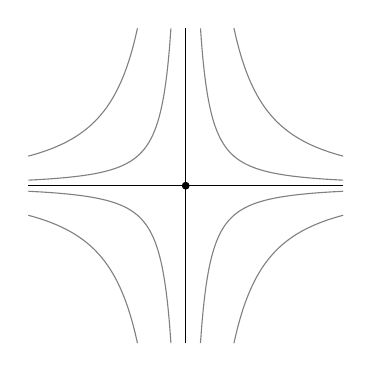
\begin{tikzpicture}
            \foreach \sx in {-0.5,0.5}
                \foreach \sy in {-0.5,0.5}
                    \draw[domain=-0.98:1.386, color=gray, smooth, variable=\t]
                        plot ({\sx*exp(\t)}, {\sy*exp(-sqrt(2)*\t)});
            \foreach \sx in {-1,1}
                \foreach \sy in {-1,1}
                    \draw[domain=-0.49:0.693, color=gray, smooth, variable=\t]
                        plot ({\sx*exp(\t)}, {\sy*exp(-sqrt(2)*\t)});
            \draw (-2,0) -- (2,0);
            \draw (0,-2) -- (0,2);
            \node[circle, fill, inner sep=1pt] at (0,0) {};
        \end{tikzpicture}
        \caption{Leaves of $xdy+\sqrt{2}ydx$.}
    \end{figure}
\end{example}

In fact, we have the following theorem (cf. \cite[Thm 2.20]{voisin_book}).

\begin{theorem}[Frobenius]\label{thm:frobenius}
    If $X$ is a smooth complex analytic variety, and $\scrF$ is a smooth
    foliation on $X$, then for any $x\in X$ there is an analytic neighbourhood
    $U$ of $x$ and a holomorphic submersion $F:U\to W\subset\C^r$ such that
    $T_\scrF|_U=\ker(dF)$.
\end{theorem}

Hence near smooth points we always have locally defined analytic leaves, given
as the fibers of a holomorphic submersion. In particular, invariant curves can
only intersect at singularities of the foliation. A key result for the local
structure at singular points is the ``separatrix theorem''.

\begin{definition}
    A \emph{separatrix} at $p\in\Sing(\scrF)$ is a local holomorphic curve $C$
    passing through $p$ and invariant under $\scrF$.
\end{definition}

\begin{theorem}[Camacho--Sad, \cite{camacho_sad_82}]\label{thm:separatrix}
    If $X$ is a smooth surface, with foliation $\scrF$, then through every
    $p\in\Sing(\scrF)$ there exists at least one separatrix.
\end{theorem}

In fact there are generalizations of this result to the case of singular $X$;
see \cref{thm:reduced separatrix}.

\begin{example}
    In \cref{ex:irrational saddle} we found two separatrices: $\{x=0\}$ and
    $\{y=0\}$.
\end{example}

% TODO: caution about global geometry of leaves, Zariski closure, torus picture

\subsection{Local analysis of singularities}

In view of \cref{thm:frobenius} the local picture of $\scrF$ at smooth points
is relatively simple, so we will be interested in the local theory of the
singular points. We will look at some invariants of the singularities of $\scrF$
which can be used to identify classes of ``nice'' singularities out of all the
possible modifications (under e.g. blowups) of a singularity, and can be
accumulated to provide some global information about $\scrF$. We will only
consider the case where the underlying surface is smooth.
 
Fix a foliation $\scrF$ on a smooth surface $X$, with a singular point
$p\in\Sing(\scrF)$. Taking local analytic coordinates $x,y$ near $p$, we have a
generator $A\pdv{}{x}+B\pdv{}{y}$ for $\scrF$.

\begin{definition}
    The \emph{multiplicity} of the singularity $p$ is
    \begin{equation*}
        m(\scrF,p)\coloneqq\dim_\C\hat\O_{X,p}/(A,B).
        % TODO: does this make sense?
    \end{equation*}
    We may then define a count of the total number of singularities of $\scrF$:
    \begin{equation*}
        m(\scrF) \coloneqq \sum_{p\in\Sing(\scrF)}m(\scrF,p),
    \end{equation*}
    which is a finite sum provided that $X$ is compact.
\end{definition}

\begin{remark}
    One could also view $m(\scrF,p)$ as the multiplicity at $p$ of the
    0-dimensional subscheme $\Sing(\scrF)\subset X$ cut out by the ideal sheaf
    in \cref{eqn:tangent sequence}.
\end{remark}

\begin{example}
    Insert example of multiplicities here.
\end{example}

% holonomy
% linearization, reduced singularities

\subsection{Blowups}

% modifications of singularities, birational geometry, see effect on local invariants, reduction to reduced singularities

% TODO: double check these

\begin{example}
    Consider the foliation given by $\omega=xdy-ydx$ on $\A^2$. % TODO: tikz

    To better deal with all these curves through the singularity, we would like
    to blow up the origin. Write $X=\Bl_{(0,0)}\A^2=U\cup V$, where
    $U=\{(x,tx,1:t)\in\A^2\times\P^1\}$, $V=\{(sy,y,s:1)\in\A^2\times\P^1\}$.
    The pullbacks to $U$ and $V$ of $\omega$ are
    \begin{equation*}
        \omega|_U = xd(tx)-txdx = x^2dt, \quad
        \omega|_V = sydy - yd(sy) = -y^2ds.
    \end{equation*}
    These vanish to second order along the exceptional divisor $E$, but
    factoring this out we get 1-forms $dt$ and $-ds$ on $U$ and $V$ which patch
    together to give a nowhere vanishing 1-form with values in the line bundle
    $\O(2E)$. (Note that $dt=-ds/s^2$, $-ds=dt/t^2$.) Pictorially this
    is exactly as expected. % TODO: tikz
\end{example}

\begin{example}
    If we instead have the singularity $\omega=xdy+ydx$, then
    \begin{equation*}
        \omega|_U = x^2dt + 2xtdx, \quad
        \omega|_V = y^2ds+2ysdy.
    \end{equation*}
    This has only first order vanishing along $E$, giving a 1-form valued in
    $\O(E)$, but with two singularities from the local forms $xdt+2tdx$,
    $yds+2sdy$. The exceptional divisor takes the role of the other separatrix
    downstairs in lifting the singularity.
\end{example}

\begin{example}\label{ex:smooth blowup}
    Finally, consider blowing up a smooth foliation; $\omega=dx$. Then
    \begin{equation*}
        \omega|_U = dx, \quad \omega|_V = sdy+yds,
    \end{equation*}
    so we have introduced a singularity on the exceptional divisor, which
    crosses the strict transform of the unique separatrix downstairs. Note that
    the pullback doesn't vanish along $E$.
\end{example}

\begin{definition}
    Suppose $(X,\scrF)$ is a foliated surface, and $p\in X$. Under the blowup
    $\pi:\tilde X=\Bl_pX\to X$ we get a rational section of
    $\pi^*N_\scrF\otimes\Omega^1_{\tilde X}$, with a pole of order $a\ge0$ on
    $E$. This then gives a section of
    $\pi^*N_\scrF(aE)\otimes\Omega^1_{\tilde X}$ defining $\tilde\scrF$, a
    foliation on $\tilde X$ with $N_{\tilde\scrF}=\pi^*N_\scrF(aE)$. Write
    $a(\scrF,p)\coloneqq a$.
\end{definition}

\begin{remark}
    The same reasoning applies to pullback a foliation along any birational
    morphism, adding exceptional divisors to the normal bundle, and more
    generally we can transport a foliation along any rational map, albeit with
    less control of the normal bundle. This is clear from the characterization
    of foliations as rational sections of $T_X$ up to multiplication by rational
    sections of $\O_X$.
\end{remark}

\begin{remark}
    By \cref{ex:smooth blowup}, we have $a(\scrF,p)=0$ for
    $p\notin\Sing(\scrF)$.
\end{remark}

\begin{theorem}[Seidenberg, \cite{seidenberg_68}]\label{thm:seidenberg}
    If $(X,\scrF)$ is a foliated surface, and $p\in\Sing(\scrF)$, then there is
    a sequence of blowups $\pi:\tilde X\to X$ of centres over $p$ such that the
    induced foliation $\tilde\scrF$ has only reduced singularities on the fiber
    over $p$.
\end{theorem}

\section{Foliations and curves} % numerical properties

Waffle about canonical bundle.

Tangency orders, vanishing orders, intersection numbers.

\section{Reduced singularities and canonical singularities}

% classification stuff

% TODO: where does this go

\begin{theorem}[Camacho, \cite{camacho_88}]\label{thm:reduced separatrix}
    Suppose $(X,\scrF)$ is a foliated surface, with a connected compact
    invariant curve $C$ satisfying
    \begin{enumerate}[label=\roman*.]
        \item The singularities of $\scrF$ meeting $C$ are reduced.
        \item The intersection matrix for $C$ is negative definite, and the dual
            graph is a tree.
    \end{enumerate}
    Then at least one of the singularities in $\Sing(\scrF)\cap C$ has a
    separatrix not contained in $C$.
\end{theorem}

\section{Examples}

% brunella' special foliation?

\section{Rational fibrations}

% TODO: look through voisin for more applications

\subsection{Rational surfaces}

\subsection{Miyaoka's criterion}

Consider a fibration $f:X\to C$ where the general fiber of $f$ is rational. For
example $X=\P^1\times\P^1$ with the projection to the first coordinate.
$K_\scrF=K_{X/C}-\{\text{effective supported on fibers}\}$,
$K_\scrF\cdot F=K_X\cdot F=-2$ for fiber $F$, $F$ nef, so for $H$ ample $nF+H$
also ample, with $K_\scrF\cdot(nF+H)=-2n+K_\scrF\cdot H<0$ for $n\gg0$.

\begin{theorem}[Miyaoka]
    Suppose $(X,\scrF)$ is a foliated surface, and $H$ is an ample divisor on
    $X$ such that $K_\scrF\cdot H<0$. Then there is a birational morphism
    $\tilde X\to X$ and a fibration $f:\tilde X\to C$ such that the general
    fiber of $f$ is rational, and $\scrF$ is the tame fibration induced by $f$.
\end{theorem}

\begin{proof}[Proof (Bogomolov, McQuillan)]
    Bertini theorem $\implies$ find $C\in|nH|$ smooth disjoint from
    $\Sing(\scrF)$. Let $Y=X\times C$. Consider the rank 1 foliation $\scrG$ on
    $Y$ given by $\scrG|_{X\times\{c\}}=\scrF$. Consider the diagonal
    $\Delta\subset C\times C\subset X\times C=Y$, which is disjoint from
    $\Sing(\scrG)$. Take the integral curves of $\scrG$ through $\Delta$ in a
    neighbourhood of $\Delta$ to define an analytic surface $S$ through
    $\Delta$. Then $N_{\Delta/S}\simeq T_\scrG|_\Delta\simeq T_\scrF|_C$, so
    $\deg N_{\Delta/S}=T_\scrF\cdot C=nT_\scrF\cdot H>0$. Hence $N_{\Delta/S}$
    is ample. It follows that $S$ is algebraic (Voisin 1st lecture). Let
    $\Sigma$ be the Zariski closure of $S$.
\end{proof}
